\documentclass{beamer}

\usetheme{LMU}

\usepackage[utf8]{inputenc}
\usepackage[T1]{fontenc}

\usepackage[english]{babel}
\usepackage{url}
%\usepackage{cite}
%\usepackage{natbib}
\usepackage[backend=bibtex,style=authoryear,dashed=false]{biblatex}
\addbibresource{../bib/eigene.bib}
\addbibresource{../bib/itip-refs.bib}
\addbibresource{../bib/other-refs.bib}
\renewcommand{\bibfont}{\normalfont\scriptsize}
\setlength{\bibhang}{3ex}

\usepackage{amssymb, amsmath, amsfonts, enumerate}
%\usepackage{bbold}
\newcommand\hmmax{0}
\usepackage{bm}
%\usepackage{dsfont}
\usepackage{pxfonts}
\usepackage{xcolor}

\usepackage{tikz}
\usetikzlibrary{%
   arrows,%
   calc,%
   fit,%
   patterns,%
   plotmarks,%
   shapes.geometric,%
   shapes.misc,%
   shapes.symbols,%
   shapes.arrows,%
   shapes.callouts,%
   shapes.multipart,%
   shapes.gates.logic.US,%
   shapes.gates.logic.IEC,%
   er,%
   automata,%
   backgrounds,%
   chains,%
   topaths,%
   trees,%
   petri,%
   mindmap,%
   matrix,%
   calendar,%
   folding,%
   fadings,%
   through,%
   patterns,%
   positioning,%
   scopes,%
   decorations.fractals,%
   decorations.shapes,%
   decorations.text,%
   decorations.pathmorphing,%
   decorations.pathreplacing,%
   decorations.footprints,%
   decorations.markings,%
   shadows}
%\usepackage{bbold}
\usepackage{hyperref}

\setbeamertemplate{blocks}[rounded][shadow=true]
\definecolor{lmugreen2}{RGB}{0,120,94}
%\definecolor{lmugreen2}{RGB}{0,148,64}
\definecolor{lmugreen}{RGB}{0,140,84}
\definecolor{unidurham}{RGB}{126,49,123}

\parindent0pt
\setlength{\unitlength}{1ex}
\setlength{\fboxsep}{0ex}

\def\then{{\color{lmugreen}$\rule[0.35ex]{2ex}{0.5ex}\!\!\!\blacktriangleright$}}
%\def\then{{\color{lmugreen}$\blacktriangleright\!\blacktriangleright$}}
%\def\then{{\color{lmugreen}$\blacktriangleright$}}
%\def\then{{\color{lmugreen}$\Rrightarrow$}}
%\def\then{{\color{lmugreen}$\rhd$}}
%\def\then{{\color{lmugreen}$\gg\!\!\!\!\!\gg$}}
%\def\then{{\color{lmugreen}${\mathbf{\gg}}$}}
\def\play{{\color{lmugreen}$\blacktriangleright$}}

\def\rthen{{\color{lmugreen}$\rule[0.35ex]{0.5ex}{0.95ex}\rule[0.35ex]{1.3ex}{0.5ex}\!\!\!\blacktriangleright$}}

\def\thenthen{{\color{lmugreen}$\blacktriangleleft\!\!\!\rule[0.35ex]{2ex}{0.5ex}\!\!\!\blacktriangleright$}}

\def\gplus{{\color{lmugreen}\rule[0.45ex]{1.4ex}{0.4ex}\hspace{-0.9ex}\rule[0.0ex]{0.4ex}{1.3ex}\hspace{0.5ex}}}
\def\gminus{{\color{lmugreen}\rule[0.45ex]{1.4ex}{0.4ex}}}


\def\blau#1{{\color{lmugreen2}#1}}
\def\rot#1{{\color{red}#1}}
\def\gruen#1{{\color{blue}#1}}
%\def\gruen#1{{\color{gray}#1}}

%%%%%%%%%%%%%%%%%%%%%%%%%%%%%%%%%%%%%%%%%
%% Definitions & shortcuts for thesis  %%
%%%%%%%%%%%%%%%%%%%%%%%%%%%%%%%%%%%%%%%%%

\def\pdc{prior-data conflict}

\newcommand{\reals}{\mathbb{R}}

\newcommand{\dd}{\,\mathrm{d}}

\newcommand{\mbf}[1]{\mathbf{#1}}
\def\bs#1{\boldsymbol{#1}}

\newcommand{\X}{\mbf{X}}
\newcommand{\x}{\mbf{x}}

\newcommand{\uz}{^{(0)}} % upper zero
\newcommand{\un}{^{(n)}} % upper n

\def\yz{y\uz}
\def\yn{y\un}

\def\yzl{\ul{y}\uz}
\def\yzu{\ol{y}\uz}

\def\ynl{\ul{y}\un}
\def\ynu{\ol{y}\un}

\def\nz{n\uz}
\def\no{n\uo}
\def\nn{n\un}

\def\nzl{\ul{n}\uz}
\def\nzu{\ol{n}\uz}

\def\nnl{\ul{n}\un}
\def\nnu{\ol{n}\un}

\def\taux{\tau(x)}
\def\ttau{\tilde{\tau}}
\def\ttaux{\ttau(x)}

\def\Y{\mathcal{Y}}
\def\YZ{\Y\uz}
\def\YN{\Y\un}
\def\N{\mathcal{N}}
\def\NZ{\N\uz}
\def\NN{\N\un}
\def\PZ{\text{I}\!\Pi\uz}
%\def\PZero{\PZ}
\def\PN{\text{I}\!\Pi\un}
\def\MZ{\mathcal{M}\uz}
\def\MN{\mathcal{M}\un}

\newcommand{\p}{\operatorname{P}}
\newcommand{\E}{\operatorname{E}}
\newcommand{\V}{\operatorname{Var}}
\newcommand{\med}{\operatorname{med}} % Median
\newcommand{\mode}{\operatorname{mode}} % Mode
\newcommand{\logit}{\operatorname{logit}} % Mode

\def\El{\ul{\E}}
\def\Eu{\ol{\E}}

\def\Pl{\ul{\p}}
\def\Pu{\ol{\p}}

\newcommand{\mult}{\operatorname{M}}    % Multinomial Distribution
\newcommand{\norm}{\operatorname{N}}    % Normal Distribution
\newcommand{\ber}{\operatorname{Ber}}   % Bernoulli Distribution
\newcommand{\bin}{\operatorname{Binom}} % Binomial Distribution
\newcommand{\be}{\operatorname{Beta}}   % Beta Distribution
\newcommand{\B}{\operatorname{B}}   % Beta Function


\def\yzr{\rot{\yz}}
\def\ynr{\rot{\yn}}
\def\byzr{\rot{\byz}}
\def\bynr{\rot{\byn}}
\def\yzor{\rot{y\uz_1}}
\def\yzjr{\rot{y\uz_j}}
\def\yzkr{\rot{y\uz_k}}
\def\yzlr{\rot{\yzl}}
\def\yzur{\rot{\yzu}}
\def\ynjr{\rot{y\un_j}}
\def\ynlr{\rot{\ynl}}
\def\ynur{\rot{\ynu}}
\def\yzjlr#1{\rot{\ul{y}\uz_#1}}
\def\yzjur#1{\rot{\ol{y}\uz_#1}}


\def\nzg{\gruen{\nz}}
\def\nng{\gruen{\nn}}
\def\nzlg{\gruen{\nzl}}
\def\nzug{\gruen{\nzu}}
\def\nnlg{\gruen{\nnl}}
\def\nnug{\gruen{\nnu}}

\def\psib{\blau{\psi}}
\def\bpsib{\blau{{b}(\psi)}}


% ------------ shading start
\newsavebox{\tempbox}
\newcommand\leftrightshading[3]{%
  \begin{tikzfadingfrompicture}[name=inputtext]
    \node [text=white] {#1};
  \end{tikzfadingfrompicture}
  \begin{lrbox}{\tempbox}%
    \begin{tikzpicture}
      \node [text=white,inner sep=0pt,outer sep=0pt] (textnode) {#1};
      \shade[path fading=inputtext,fit fading=false,left color=#2,right color=#3]
      (textnode.south west) rectangle (textnode.north east);
    \end{tikzpicture}%
  \end{lrbox}
  % Now we use the fading in another picture:
  \usebox\tempbox{}%
}
% ------------ shading end


%\def\PZc{\mathrm I\!\Pi\uz}
\def\PZc{\leftrightshading{$\mathrm I\!\Pi\uz$}{blue}{red}}
%\def\PNc{\PN}
\def\PNc{\leftrightshading{$\mathrm I\!\Pi\un$}{blue}{red}}


\title%[]
{Prior-Data Conflict\\ in Generalised Bayesian Inference}

\author%[]
       {Gero Walter}

\institute{Department of Statistics\\
           Ludwig-Maximilians-Universit\"at M\"unchen (LMU)\\
                      {}%\{gero.walter; thomas\}@stat.uni-muenchen.de
}

\date{September 16th, 2013}


\titlegraphic{
%\begin{center}
\includegraphics[scale=0.032]{lmu_logos/lmu_massiv.png}
\raisebox{1.375cm}{
\includegraphics[scale=0.4]{lmu_logos/lmu_statistic.pdf}
}
%\end{center}
}

\begin{document}


\frame{
\titlepage
}

\frame{\frametitle{Outline}
\begin{enumerate}
\item Bayesian inference \& prior-data conflict %and Strong prior-data agreement\\ (joint work with Thomas Augustin and Frank Coolen)
\item Generalised Bayesian inference with sets of priors\\ (joint work with Thomas Augustin)
\item Common-cause failure modeling\\ (joint work with Matthias Troffaes and Dana Kelly)
\end{enumerate}
}

\section{Prior-Data Conflict}

\subsection{Bayesian Inference}

\frame{\frametitle{Bayesian Inference \& Prior-Data Conflict}

\uncover<1->{%
\begin{block}{The Bayesian approach to statistical inference}
\centerline{prior $p(\vartheta)$ + likelihood $f(\x\mid\vartheta)$\hspace*{1ex} \then\ \ posterior $p(\vartheta\mid\x)$}
%\quad using Bayes' Rule}
All inferences are based on the posterior (e.g., point estimate, \ldots)
\end{block}}
\uncover<2->{%
Assigning a certain prior distribution on $\vartheta$\\
\hfill $=$ defining a conglomerate of probability statements (on $\vartheta$).
}
\uncover<3->{%
\begin{block}{Prior-Data Conflict}
\begin{itemize}
\item \emph{informative prior beliefs} and \emph{trusted data}\\ %\rule{0ex}{3ex}\\
(sampling model correct, no outliers, etc.) are in conflict%\\%[2ex]
\item ``[\ldots] the prior [places] its mass primarily on distributions
in the sampling model for which the observed data is surprising''\\
(Evans \& Moshonov, 2006)
\item there are not enough data to overrule the prior
\end{itemize}
\end{block}}

%\uncover<2->{%
%example for application where \pdc\ is relevant:\\ %can show up:\\
%\alert{common-cause failure modeling} (more later)
%}

}


\subsection{Basic Example}

\frame{\frametitle{Prior-Data Conflict: Basic Example}

%Example Beta-Binom, show point, line, rectangle
\begin{itemize}[<+->]
\item Bernoulli observations: 0/1 observations (team wins no/yes)
\item given: a set of observations and strong prior information
%\item given: a set of observations (team won 12 out of 16 matches)
%\item additional to observations, we have strong prior information\\ (we are convinced that $P(\text{win})$ should be around $0.75$)
\item we are, e.g., interested in (predictive) probability $P$ that team wins in the next match
%(or some other inferences) %(predictive probability!)
%\item standard statistical model for this situation: Beta-Bernoulli/Binomial Model
%\item \textbf{\pdc:} if $P(\text{heads})$ for the coin is actually very different from our prior guess
%(i.e., prior information and data are in conflict), this should show up in the %predictive
%inferences (probability $\mbox{P}$ and, e.g., confidence intervals)
\end{itemize}
\uncover<4->{
\begin{block}{Beta-Binomial Model}
\begin{tabular}{r|lcl}
data :           & $s\mid \theta$          & $\sim$ & $\bin(n,\theta)$   \\[0.5ex]
conjugate prior: & $\theta\mid \nzg, \yzr$ & $\sim$ & $\be(\nzg,\, \yzr)$  \\[0.5ex]
\cline{1-4}
posterior:       & $\theta\mid \nng, \ynr$ & $\sim$ & $\be(\nng,\, \ynr)$\rule{0ex}{2.5ex}
%\quad ($\frac{\tau(\x)}{n} = \frac{s}{n}$)\rule{0ex}{2.5ex}
\end{tabular}
\end{block}
where $s$ = number of wins in the $n$ matches observed
}

}

\subsection{Beta-Binomial Model}

\frame{\frametitle{Beta-Binomial Model}

\uncover<1->{
\begin{block}{Beta-Binomial Model}
\begin{tabular}{r|lcl}
data :           & $s\mid \theta$          & $\sim$ & $\bin(n,\theta)$   \\[0.5ex]
conjugate prior: & $\theta\mid \nzg, \yzr$ & $\sim$ & $\be(\nzg,\, \yzr)$  \\[0.5ex]
\cline{1-4}
posterior:       & $\theta\mid \nng, \ynr$ & $\sim$ & $\be(\nng,\, \ynr)$\rule{0ex}{2.5ex}
%\quad ($\frac{\tau(\x)}{n} = \frac{s}{n}$)\rule{0ex}{2.5ex}
\end{tabular}
\end{block}
}
\begin{align*}
\uncover<2->{%
P = \E[\theta\mid\nng,\ynr]
}%
\uncover<3->{%
= \rot{\yn}
= \frac{\gruen{\nz}}{\gruen{\nz} + n} \cdot \rot{\yz} + \frac{n}{\gruen{\nz} + n} \cdot \frac{s}{n}
}%
\end{align*}\vspace*{-3ex}
\begin{align*}
\uncover<4->{%
\gruen{\nn} &= \gruen{\nz} + n
}%
\uncover<5->{%
& \V(\theta\mid\nng,\ynr) &= \frac{\rot{\yn}(1-\rot{\yn})}{\gruen{\nn} + 1}
}
\end{align*}

}

\frame{\frametitle{Beta-Binomial Model (BBM)}

\hspace*{-12ex}
\begin{columns}%[T]
\begin{column}{0.55\textwidth}
\begin{tikzpicture}
\pgftransformscale{0.025}
\uncover<1>{
\input{precise01.tex}
}
\uncover<2>{
\input{precise02.tex}
\draw[-stealth,very thick] (110,175) -- (220,175) node [above,midway] {12 out of 16};
}
\uncover<3->{
\input{precise03.tex}
\draw[-stealth,very thick,gray] (110,175) -- (220,175) node [above,midway,gray] {12 out of 16};
}
\uncover<4->{
\draw[-stealth,very thick] (110,102) -- (220,167) node [above,midway,sloped] {16 out of 16};
}
\uncover<5>{%
%\draw[thick,fill=white] (0,0) rectangle (100,50) {text};
%\node at (140,80) {\parbox{0.5\textwidth}{
\draw (160,35) node [rectangle,very thick,draw,fill=white] {\parbox{23.5ex}{
%\begin{block}{}
Weighted average structure\\ is underneath \alert{all common\\ conjugate priors}
for\\ exponential family\\ sampling distributions!
%\end{block}
}};
} %
\end{tikzpicture}
\end{column}
\begin{column}{0.45\textwidth}
\uncover<1->{%
\begin{block}{no conflict:}
prior $\nzg = 8$, $\yzr = 0.75$\\
data $s/n = 12/16 = 0.75$
\end{block}
} %
\uncover<2->{%
\vspace*{-1.5ex}\centerline{\color{lmugreen} $\blacktriangledown$}\vspace*{-1.5ex}
\begin{block}{}
$\nng = 24$, $\ynr = 0.75$
\end{block}
} %
\uncover<4->{%
\vspace*{-1.5ex}\centerline{\color{lmugreen} $\blacktriangle$}\vspace*{-1.5ex}
}
\uncover<3->{%
\begin{block}{\pdc:}
prior $\nzg = 8$, $\yzr = 0.25$\\
data $s/n = 16/16 = 1$
\end{block}
} %
\uncover<0>{%
\vspace*{-1.5ex}\centerline{\color{lmugreen} $\blacktriangledown$}\vspace*{-1.5ex}
\begin{block}{}
$\nng \in [20, 24]$, $\ynr \in [0.73, 0.86]$
\end{block}
} %
%\uncover<5->{ %
%\then\ same predictive prob.\ P!
%}
\end{column}
\end{columns}

}

\iffalse
\subsection{Canonical Conjugate Priors}

\frame{\frametitle{Canonical Conjugate Priors}

\uncover<1->{%
%The multinomial is an example for a \alert{canonical exponential family} %(Bernardo \& Smith, 2000)
Weighted average structure is underneath \alert{all common conjugate priors}
for exponential family sampling distributions! %\\[2ex]

\begin{block}%
{$(x_1, \ldots, x_n) = \x \stackrel{iid}{\sim}$ canonical exponential family} %(Bernardo and Smith, 1994)
%, i.e.
\begin{align*}
p(\x \mid \vartheta) &\propto \exp\big\{\langle \psib, \tau(\x) \rangle - n \bpsib \big\}
\qquad \Big[ \psib \text{ transformation of } \vartheta \Big]
\end{align*}
(includes Binomial, Multinomial, Normal, Poisson, Exponential, \ldots )%\\[2ex]
\end{block}}
\vspace*{-3ex}%
\begin{align*}
\uncover<2->{%
&\text{\play\ conjugate prior:} &
p(\psib\mid\nzg,\yzr) \hspace*{2ex}
&\propto \exp\big\{ \nzg \big[\langle \psib, \yzr \rangle - \bpsib\big]\big\} \\}
\uncover<3->{%
&\text{\play\ (conjugate) posterior:} &
p(\psib\mid\nzg,\yzr,\vec{x})
%p(\psib\mid\nng,\ynr) \hspace*{2ex}
&\propto \exp\big\{ \nng \big[\langle \psib, \ynr \rangle - \bpsib\big]\big\} }%\quad \mbox{where}
\end{align*}
\begin{align*}
\uncover<3->{%
\mbox{where}\quad \ynr &= \frac{\nzg}{\nzg + n} \cdot \yzr + \frac{n}{\nzg + n} \cdot \frac{\tau(\x)}{n}
& &\mbox{and} & \nng &= \nzg + n }
\end{align*}

}


\frame{\frametitle{Canonical Conjugate Priors}

\vspace*{-2ex}%
\uncover<1->{%
\begin{align*}
&\text{\play\ (conjugate) posterior:} &
%p(\psib\mid\nzg,\yzr,\vec{x})
p(\psib\mid\nng,\ynr) %\hspace*{2ex}
&\propto \exp\big\{ \nng \big[\langle \psib, \ynr \rangle - \bpsib\big]\big\} %\quad \mbox{where}
\end{align*}
\vspace*{-2ex}
\begin{align*}
\mbox{where}\quad \ynr &= \frac{\nzg}{\nzg + n} \cdot \yzr + \frac{n}{\nzg + n} \cdot \frac{\tau(\x)}{n}
& &\mbox{and} & \nng &= \nzg + n
\end{align*}}%
\vspace*{-2ex}%
\uncover<2->{%
\begin{block}{Interpretation}
  \begin{itemize}
  \item $\nzg$ = determines \alert{spread} and \alert{learning speed}
  \item $\yzr$ = \alert{prior expectation} of $\tau(\x)/n$ %$\frac{\tau(\vec{x})}{n}$
  \end{itemize}
\end{block}}%
\uncover<3->{%
\begin{block}{Example: Scaled Normal Data}
\begin{tabular}{r|lcl}
Data :           & $\x\mid\mu$        & $\sim$ & $\norm(\mu,1)$\\[0.5ex] %\sigma_0^2)$ \quad ($\sigma_0^2$ known)\\[0.5ex]
conjugate prior: & $\mu\mid\nzg,\yzr$ & $\sim$ & $\norm(\yzr, 1/\nzg)$  \\[0.5ex]
\cline{1-4}
posterior:       & $\mu\mid\nng,\ynr$ & $\sim$ & $\norm(\ynr, 1/\nng)$ \quad ($\frac{\tau(\x)}{n} = \bar{\x}$)\rule{0ex}{2.5ex} %& \\[0.5ex]
\end{tabular}
\end{block}}
}
\fi


\section{Generalised Bayesian Inference}

\subsection{Why Generalise Bayesian Inference?}

\frame{\frametitle{Why Generalise Bayesian Inference?}

%Weighted average structure is underneath \alert{all common conjugate priors}
%for exponential family sampling distributions!\\[1.5ex]

%\pause
Bayesian theory lacks the ability to specifiy the degree of uncertainty in probability statements
encoded in a (prior, posterior) distribution.\\[1.5ex]

\pause
Variance or stretch of a distribution for describing uncertainty?\\[1.5ex]
%but this mostly does not work in conjugate updating as just shown.
%but this has mostly no influence on the behaviour to prior-data conflict.

\pause
\then\ \parbox[t]{0.9\textwidth}{Does not work in the case of prior-data conflict:\\
In conjugate updating, the posterior variance does not depend
on the degree of prior-data conflict in most cases.}\\[1.5ex]

\then\ How to express the precision of a probability statement?\\

}

\frame{\frametitle{Imprecision}

%\hspace*{6ex}\parbox[t]{0.9\textwidth}{
\textbf{Add \alert{imprecision} as new model dimension:\\
\alert{Sets of priors} model uncertainty in probability statements}\\[2ex]
%}

\uncover<2->{%
\begin{block}{Interpretation}
\centerline{smaller sets \thenthen\ more precise probability statements}
\vspace*{1ex}
\parbox[t]{0.45\textwidth}{\centering \textbf{Lottery A}\\
                          Number of winning tickets:\\
                          exactly known as 5 out of 100\\
                          \then\ $P(\text{win}) = 5/100$}
\qquad
\parbox[t]{0.45\textwidth}{\centering \textbf{Lottery B}\\
                          Number of winning tickets:\\
                          not exactly known, supposedly\\
                          between 1 and 7 out of 100\\
                          \then\ $P(\text{win}) = [1/100,\, 7/100]$}
\end{block}
}
%\uncover<3->{%
%\centerline{shorter intervals \thenthen\ more precise probability statements}
%}
}

\subsection{Sets of Priors}

\frame{\frametitle{Bayesian Inference with Sets of Priors}

\uncover<1->{%
\begin{block}{Standard Bayesian inference procedure}
\centerline{prior + likelihood\hspace*{1ex} \then\ \ posterior}
using Bayes' Rule\\
All inferences are based on the posterior%\\
%(e.g., point estimate = $\E[\psib\mid\nng,\ynr]$)
\end{block}}

\uncover<2->{%
\begin{block}{Generalised Bayesian inference procedure}
\centerline{set of priors + likelihood\hspace*{1ex} \then\ \ set of posteriors}
All inferences are based on the set of posteriors\\
\emph{Coherence} (consistency of inferences) ensured by using\\
\emph{Generalised Bayes' Rule} (GBR, Walley 1991)\\
= element-wise application of Bayes' Rule\\ %\emph{\small (set of priors must be convex)}\\
%(e.g., point estimate = $\big[\El[\psib\mid\nng,\ynr],\Eu[\psib\mid\nng,\ynr]\big]$)
\end{block}}

\uncover<3->{\centerline{Let hyperparameters $(\nzg, \yzr)$ vary in a set $\PZc$ \then\ \alert{set of priors}}}

}

\iffalse
\frame{\frametitle{Generalised Bayesian Inference Procedure}

\vspace*{-1ex}%
\uncover<1->{%
\begin{align*}
\text{single prior $(\nzg, \yzr)$}
 &\quad\mbox{\then }\quad 
\text{set of priors $\MZ$ (defined via $\PZc$)} \\
\E[\psib\mid\nzg,\yzr,\x]
 &\quad\mbox{\then }\quad 
\big[\El[\psib\mid\PZc,\x],\Eu[\psib\mid\PZc,\x]\big] \\
P(\psib\in A\mid\nzg,\yzr,\x)
 &\quad\mbox{\then }\quad 
\big[\Pl[\psib\in A\mid\PZc,\x],\Pu[\psib\in A\mid\PZc,\x]\big]
%\E[\theta]  &\quad\mbox{\then }\quad \big[\LE[\theta],\, \UE[\theta]\big] \\
%= \left[ \min_{p \in {\cal M}_\theta} \E_{p}[\theta],\,
%         \max_{p \in {\cal M}_\theta} \E_{p}[\theta]\right]\\
%P(\theta\! \in\! A) &\quad\mbox{\then }\quad \big[\ul{P}(\theta\! \in\! A),\, \ol{P}(\theta\! \in\! A)\big]
%= \big[\! \min P_{\!\!p}(\theta\! \in\! A),\,
%          \max P_{\!\!p}(\theta\! \in\! A)\big]
\end{align*}
\begin{center}
Lower/upper posterior expectation by min/max over set of posteriors %$\PZc$
\end{center}}
\uncover<2->{%
\begin{block}{Interpretation}
\centerline{\textbf{Shorter intervals \thenthen\ more precise probability statements}}
\vspace*{1ex}
\parbox[t]{0.45\textwidth}{\centering \textbf{Lottery A}\\
                          Number of winning tickets:\\
                          exactly known as 5 out of 100\\
                          \then\ $P(\text{win}) = 5/100$}
\qquad
\parbox[t]{0.45\textwidth}{\centering \textbf{Lottery B}\\
                          Number of winning tickets:\\
                          not exactly known, supposedly\\
                          between 1 and 7 out of 100\\
                          \then\ $P(\text{win}) = [1/100,\, 7/100]$}
\end{block}}

}
\fi


%\frame{\frametitle{Imprecise BBM with $\nzg$ fixed = IDM (Walley 1996)}
\frame{\frametitle{Imprecise BBM with $\nzg$ fixed: \parbox{0.44\textwidth}{\small IDM (Walley 1996)\\ Quaghebeur \& de Cooman (2005)}}
\hspace*{-12ex}
\begin{columns}%[T]
\begin{column}{0.55\textwidth}
\begin{tikzpicture}
\pgftransformscale{0.025}
\uncover<1>{
\input{line01.tex}
}
\uncover<2>{
\input{line02.tex}
\draw[-stealth,very thick] (110,175) -- (220,175) node [above,midway] {12 out of 16};
}
\uncover<3->{
\input{line03.tex}
\draw[-stealth,very thick,gray] (110,175) -- (220,175) node [above,midway,gray] {12 out of 16};
}
\uncover<4->{
\draw[-stealth,very thick] (110,102) -- (220,167) node [above,midway,sloped] {16 out of 16};
}
\end{tikzpicture}
\end{column}
\begin{column}{0.45\textwidth}
\uncover<1->{%
\begin{block}{no conflict:}
prior $\nzg = 8$, $\yzr \in [0.7, 0.8]$\\
data $s/n = 12/16 = 0.75$
\end{block}
} %
\uncover<2->{%
\vspace*{-1.5ex}\centerline{\color{lmugreen} $\blacktriangledown$}\vspace*{-1.5ex}
\begin{block}{}
$\nng = 24$, $\ynr \in [0.73, 0.77]$
\end{block}
} %
\uncover<4->{%
\vspace*{-1.5ex}\centerline{\color{lmugreen} $\blacktriangle$}\vspace*{-1.5ex}
}
\uncover<3->{%
\begin{block}{\pdc:}
prior $\nzg = 8$, $\yzr \in [0.2, 0.3]$\\
data $s/n = 16/16 = 1$
\end{block}
} %
\uncover<0>{%
\vspace*{-1.5ex}\centerline{\color{lmugreen} $\blacktriangledown$}\vspace*{-1.5ex}
\begin{block}{}
$\nng \in [20, 24]$, $\ynr \in [0.73, 0.86]$
\end{block}
} %
%\uncover<5->{ %
%\then\ same imprecise predictive prob.\ $[\Pl,\Pu]$!
%}
\end{column}
\end{columns}

}


\frame{\frametitle{Imprecise BBM with $[\nzlg,\nzug]$: \parbox{0.43\textwidth}{\small Walley (1991, \S 5.4.3)\\ Walter \& Augustin (2009)}}
\hspace*{-12ex}
\begin{columns}%[T]
\begin{column}{0.55\textwidth}
\begin{tikzpicture}
\pgftransformscale{0.025}
\uncover<1>{
\input{rect01.tex}
}
\uncover<2>{
\input{rect02.tex}
\draw[-stealth,very thick] (110,175) -- (193,175) node [above,midway] {12 out of 16};
}
\uncover<3>{
\input{rect03.tex}
\draw[-stealth,very thick,gray] (110,175) -- (193,175) node [above,midway,gray] {12 out of 16};
}
\uncover<4>{
\input{rect04.tex}
\draw[-stealth,very thick,gray] (110,175) -- (193,175) node [above,midway,gray] {12 out of 16};
\draw[-stealth,very thick] (110,102) -- (213,180) node [above,midway,sloped] {16 out of 16};
%\draw[-stealth,very thick, postaction={decorate,decoration={raise=2pt,text along path, %
%                                       text={16 out of 16}}}] (110,95) .. controls +(right:30) and +(down:30) .. (210,183);
%\draw[-stealth,very thick] (110,95) .. controls +(right:10) and +(down:10) .. (210,183) node [below,midway,sloped] {16 out of 16};
}
\end{tikzpicture}
\end{column}
\begin{column}{0.45\textwidth}
\uncover<1->{%
\begin{block}{no conflict:}
prior $\nzg\! \in [4, 8]$, $\yzr\! \in [0.7, 0.8]$\\
data $s/n = 12/16 = 0.75$
\end{block}
} %
\uncover<2->{%
\vspace*{-1.5ex}\centerline{\color{lmugreen} $\blacktriangledown$}\vspace*{-1.5ex}
\begin{block}{}
%$\gruen{\nn} \in [20, 24]$,
\centering $\ynr \in [0.73, 0.77]$
%\centering ``spotlight'' shape
\end{block}
} %
\uncover<3->{%
\begin{block}{\pdc:}
prior $\nzg \in\! [4, 8]$, $\yzr\! \in [0.2, 0.3]$\\
data $s/n = 16/16 = 1$
\end{block}
} %
\uncover<4->{%
\vspace*{-1.5ex}\centerline{\color{lmugreen} $\blacktriangledown$}\vspace*{-1.5ex}
\begin{block}{}
%$\gruen{\nn} \in [20, 24]$,
\centering $\ynr \in [0.73, 0.86]$
%\centering ``banana'' shape
\end{block}
} %
\end{column}
\end{columns}

}


\subsection{Parameter Set Shapes}

\frame{\frametitle{Parameter Set Shapes}

\begin{itemize}%[<+->]
\item<1-> $\PZc = \nzg \times [\yzlr, \yzur]$:\\% \thenthen\
IDM (Walley 1996), Quaghebeur \& de Cooman (2005)
 \begin{itemize}%[<+->]
 \item posterior parameter set has same form $\PNc = \nng \times [\ynlr, \ynur]$ %simpel model description,
 \item optimise over $[\ynlr, \ynur]$ only %(often, posteriors are stoch.\ ordered along $\ynr$)
 \item no \pdc\ reaction: same imprecision as without conflict (just like precise priors)
 \end{itemize}
\item<2-> $\PZc = [\nzlg,\nzug] \times [\yzlr, \yzur]$: %\thenthen\
Walley (1991, \S 5.4.3),\\ \emph{generalised iLUCK-models} (Walter \& Augustin 2009) 
 \begin{itemize}%[<+->]
 \item still simple to elicit, allows flexible weighing of prior and data
 \item additional imprecision in case of \pdc\\ \then\ more cautious inferences
 \item $\PNc$ have non-trivial forms (banana / spotlight) %posterior parameter sets 
 \item however, closed form for $\min / \max \ynr$ over $\PNc$
 \item general optimisation over $\PNc$ more difficult, but doable
 \item \textbf{R} package \texttt{luck}: do optimisation over $\PZc$ actually 
 \end{itemize}
\end{itemize}

}


%\frame{\frametitle{Parameter Set Shapes: Discussion}
\frame{\frametitle{Model Summary}

%\begin{itemize}[<+->]
%\item Shape of $\PZc$ influences shape of $\PNc$
%\item Shape of $\PNc$ influences model behaviour\\
%\then\ shape of $\PZc$ is a crucial modelling choice
%\item $\PZc = [\nzlg, \nzug] \times [\yzlr, \yzur]$ (\emph{rectangle}) %(as before)
%is very easy to elicit\\
%and gives good model behaviour for \alert{\pdc}
%\end{itemize}

\begin{itemize}%[<+->]
\item<1-> Easy to handle, generally favourable inference properties, e.g.:\\
$n \to \infty$\hspace*{0.9ex}%
%\uncover<2->{\then\ \ $\ynr$ values in $\PNc \to \frac{\tau(\x)}{n}$\hspace*{0.9ex}}%
%\uncover<3->{\then\ \ `Bayesian consistency'}
\uncover<2->{\then\ \ $\ynr$ stretch in $\PNc \to 0$\hspace*{0.9ex}}%
\uncover<3->{\then\ \ more precise inferences}
\item<4-> A range of $\nzg$ values is needed for \pdc\ reaction
\item<5-> Other set shapes are possible, but may be more difficult to elicit
\item<6-> Prior information may be such that range of $\yzr$ changes with $\nzg$ (or vice versa)
\item<7-> Work in progress (joint work with Frank Coolen):\\
parameter set shape enabling\ldots
\begin{itemize}
\item additional imprecision in case of \pdc\ (as before)
\item less imprecision for \emph{strong prior-data agreement}
\end{itemize}
%This work uses 
via a different parametrisation of priors suggested by Mi\c{k} Bickis % (in preparation)
\end{itemize}

}

\frame{\frametitle{Parameter Set Shapes: Outlook}

%\hspace*{-2ex}%
%\uncover<2->{%
%\vspace*{-7ex}%
\begin{center} %trim=l b r t
%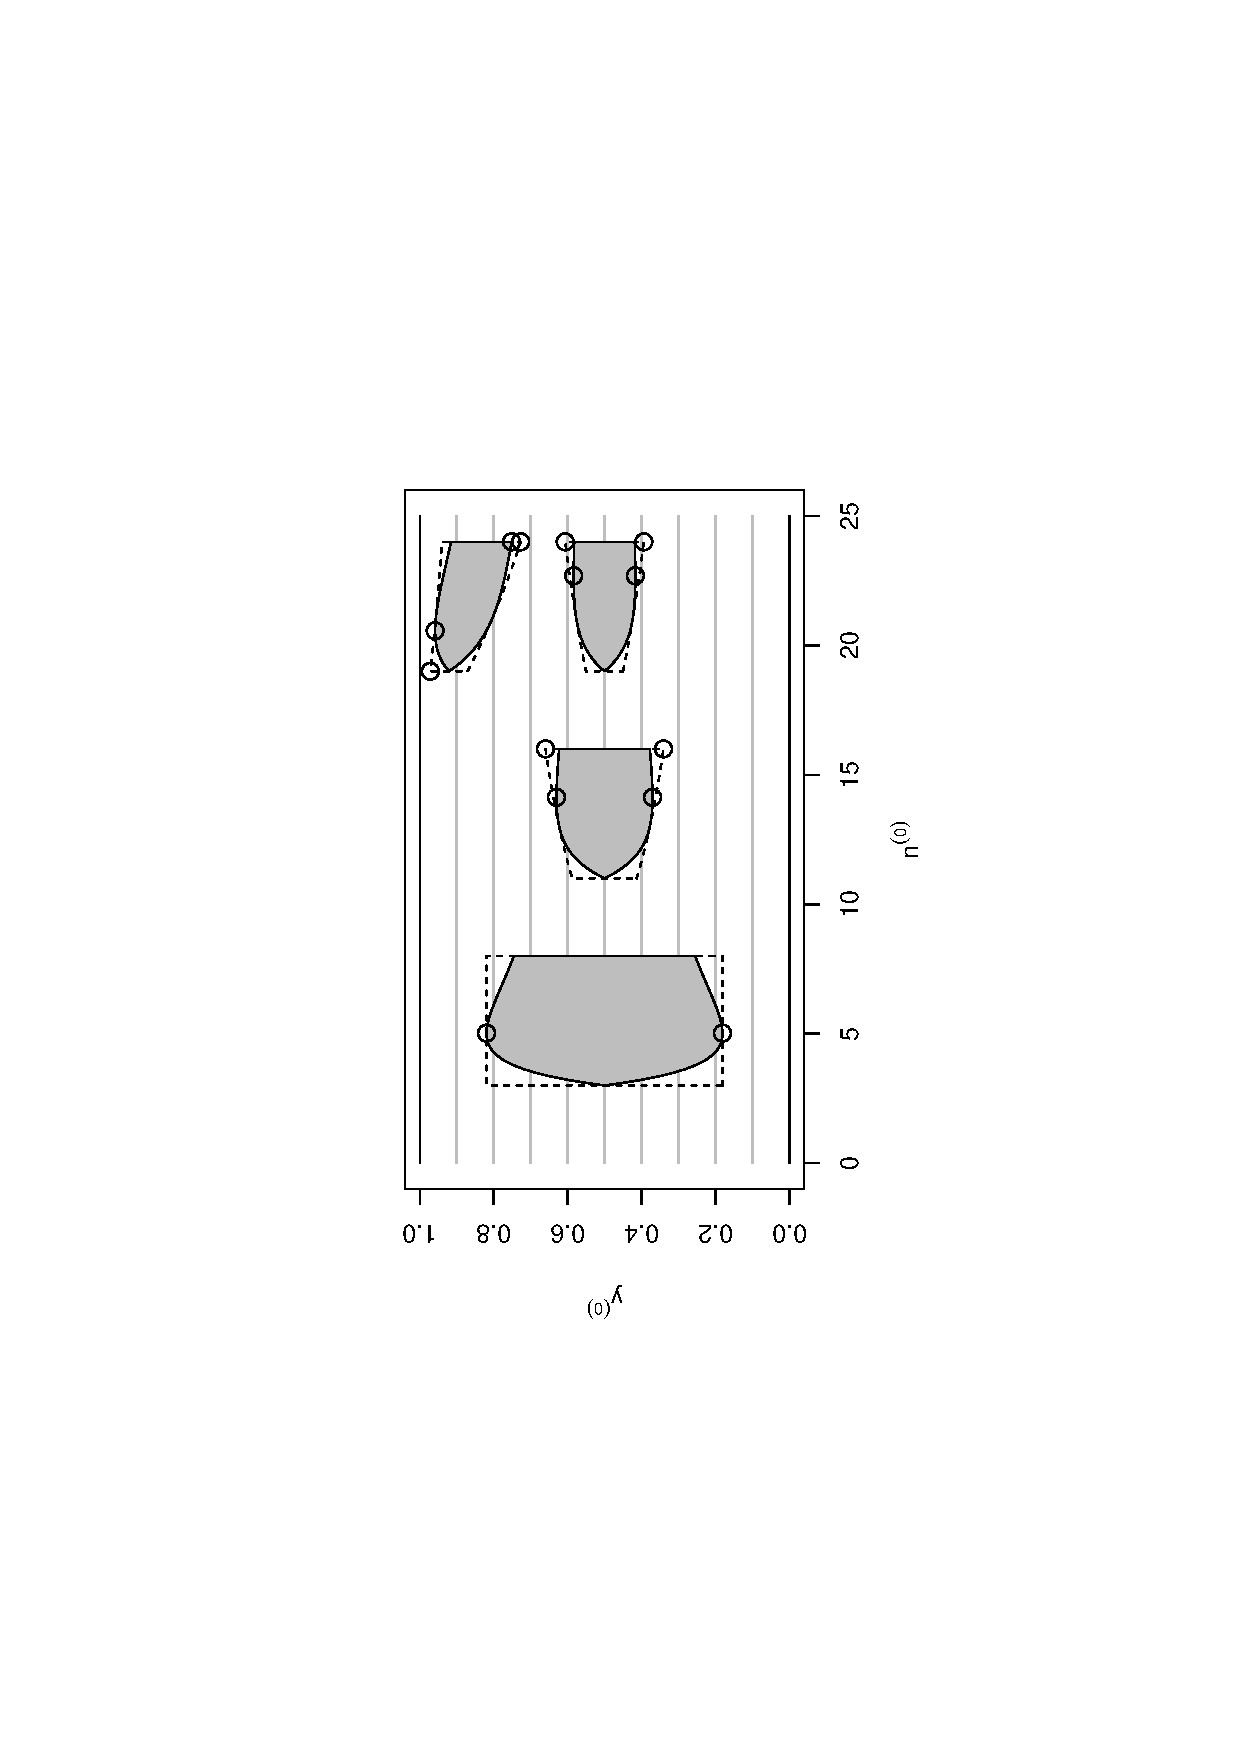
\includegraphics[trim = 40mm 35mm 40mm 45mm, clip, width=\textwidth]{../R/boatshape-durham0913} % width=8, height=6
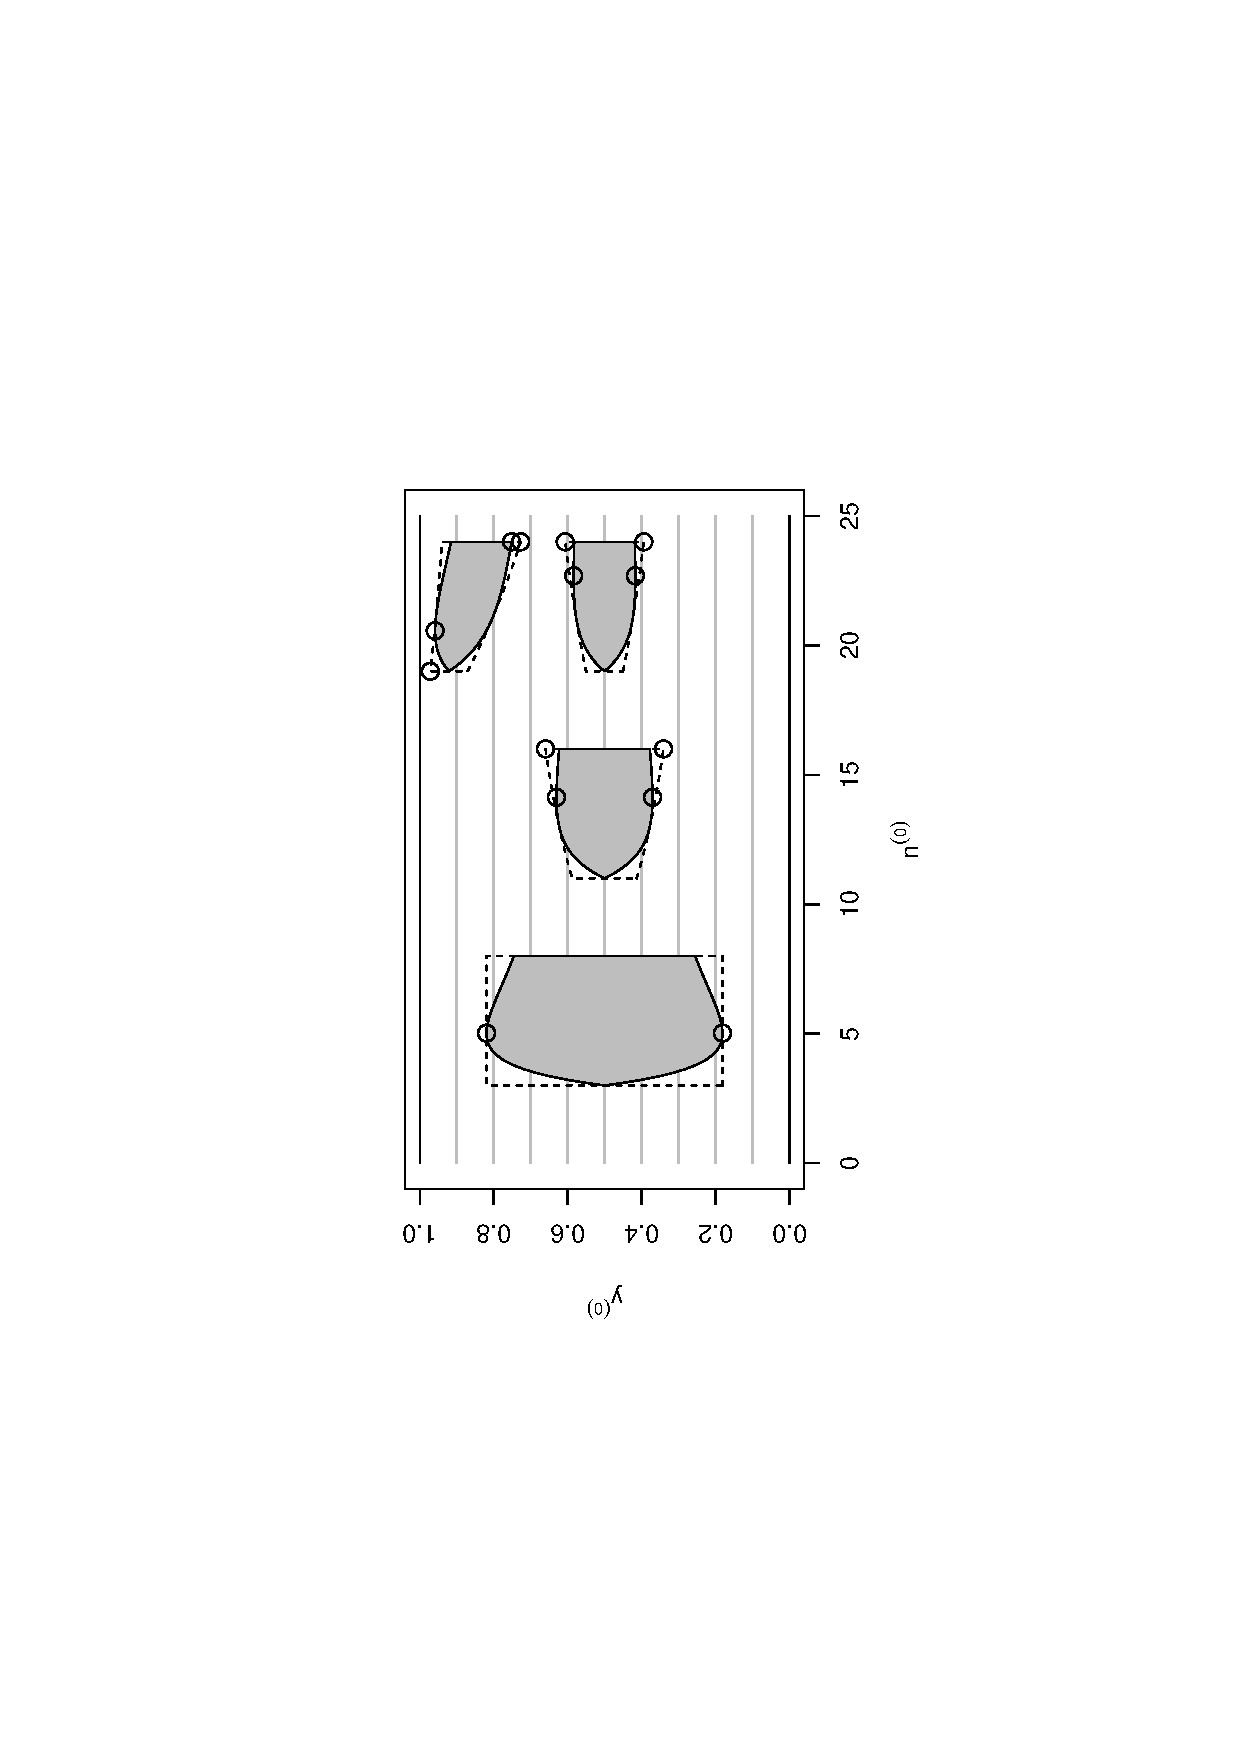
\includegraphics[trim = 70mm 52.5mm 70mm 65mm, clip, width=\textwidth]{../R/boatshape-durham0913} % width=6, height=4.5
\end{center}%}

}


\section{Common-Cause Failure Modeling}

\subsection{Common-Cause Failures}

\frame{\frametitle{Common-Cause Failures}
\begin{tikzpicture}
\uncover<1->{
\node {\includegraphics[scale=0.4]{./graph/800px-Fukushima_I_by_Digital_Globe.jpg}};
\node at (0,-3.5) {\tiny Source: Wikimedia Commons, \url{http://commons.wikimedia.org/wiki/File:Fukushima_I_by_Digital_Globe.jpg}};
}
\uncover<2->{
%\draw[white,fill=white] (-5,1) rectangle (5,3);
\node at (0,2.6) {\parbox{\textwidth}{
 \begin{alertblock}{common-cause failure} 
 \emph{simultaneous failure of several redundant components\\ due to a common or shared root cause}
 (H{\o}yland \& Rausand, 1994)
 \end{alertblock}
}};
}
\uncover<3>{
\draw[white,fill=white] (-0.2,-3.3) rectangle (6,0.75);
\node at (3,-1) {\includegraphics[scale=0.3]{./graph/plant-systems-diesel-generator.jpg}};
\node at (3.05,-3.05) {\parbox{6.2cm}{\tiny Source: \url{http://www.diakont.com/solutions/nuclear-energy/plant-systems/diesel-generator-control-systems/}}};
}
\end{tikzpicture}
}

\frame{\frametitle{Common-Cause Failure Modeling}


\begin{itemize}[<+->]
\item Crucial for overall system reliability analysis
\item \alert{Alpha factor model} is based on the Dirichlet-Multinomial model:\\
{\small categories $1,2,3,\ldots = 1,2,3,\ldots$ components failing simultaneously}
\item Informative Dirichlet priors elicited from experts\\ as data are sparse (zero counts for multi-component failures)
\item Non-informative priors are unsatisfactory:
 \begin{itemize}
 \item posterior is very sensitive to choice of prior
 \item which non-informative prior should we adopt?
 \end{itemize}
\item Troffaes, Walter \& Kelly (2013): sets of Dirichlet priors %(IDM, Walley 1996)
%\item Prior-data conflict sensitivity especially important for multi-component failures
\item More cautious inferences if prior and data are in conflict\\
(especially important for multi-component failures!)
\item Simple ways to elicit bounds for hyperparameters\\ by reasoning on hypothetical data
\end{itemize}

}

\subsection{Conclusion}

\frame{\frametitle{Conclusion}

\begin{itemize}%[<+->]
\item<1-> Conjugate priors are a convenient tool for Bayesian inference\\ but there are some pitfalls
 \begin{itemize}%[<+->]
 \item Hyperparameters $\nzg,\yzr$ are easy to interpret and elicit
 \item Averaging property makes calculations simple, but leads to
 inadequate model behaviour in case of \pdc
 \end{itemize}
\item<2-> Sets of conjugate priors maintain advantages \& mitigate issues %find a sweet spot in between
 \begin{itemize}%[<+->]
 \item Hyperparameter set shape is important %a crucial modeling choice
 \item Reasonable choice: \emph{rectangular} $\PZc = [\nzlg, \nzug] \times [\yzlr, \yzur]$
 \item Bounds for hyperparameters easy to interpret and elicit
 \item Additional imprecison in case of \pdc\\
 leads to \alert{cautious inferences if, and only if, caution is needed}
 \item Shape for more precision in case of strong prior-data agreement is in development
 (joint work with Frank Coolen and Mi\c{k} Bickis)
 \end{itemize}
\end{itemize}

}


\frame{\frametitle{References}

\nocite{2006:evans,1996:walley::idm,1991:walley,2005:quaeghebeurcooman-short,
Walter2009a-short,luck-package,Troffaes2013a,1994:hoyland,2012:benavolizaffalon-short}
%1965:good,2011:kelly:atwood,1996:atwood,}

\printbibliography[heading=none]

%\bibliographystyle{plainnat}
%\bibliography{../bib/eigene,../bib/itip-refs,../bib/other-refs}
}

\end{document}
